\section{System Overview (75 pts)}

\subsection{System In A Nutshell}

In this project we created a middleware-based key-value store system, which consists of three components: the memtier clients, the middleware, and the memcached servers.

The memtier clients set and retrieve key-value pairs by continuously sending requests to the server and port specified in its startup arguments. The request format complies to the memcached protocol \footnote{https://github.com/memcached/memcached/blob/master/doc/protocol.txt}. A memtier instance runs with multiple threads, and each thread works as multiple virtual clients: a client sends requests one by one, i.e. it will not send a new request until it has received the response of its last request.

The middleware relays requests and responses between clients to memcached servers, and balances the load. From a client's point of view, it is transparent and behaves in the same way as a memcached server would do. The middleware can receive connections from multiple clients, forward their requests to one or more servers depending on the request type, and send the responses of servers to the corresponding clients. With a multi-threaded architecture, multiple workers can concurrently process multiple requests.

The memcached server listens on a port by both TCP and UDP, and can keep many client connections simultaneously. It can work with multiple threads, but in this project we only use one. It supports a variety of request types, such as storage, retrieval and statistics commands, while in this project we only consider \texttt{GET}s and \texttt{SET}s. 

To deploy the system, a Microsoft Azure cluster with eight virtual machines is used, of which the configurations are shown in Table~\ref{table:azure_config}. The upload and download bandwidths are measured with \texttt{iperf}, each with three repetitions, so both the averages and the standard deviations (in brackets) are listed. To measure the download bandwidth of one virtual machine, it is configured as \texttt{iperf} server, and all other machines are setup as clients to send traffic simultaneously to it. Due to various factors of data center VM allocation, and the limit of individual client's upload bandwidth, they together may still not hit the server's true download limit, so the measured value is only the highest lower bound that can be observed. For upload bandwidth, a machine is configured as \texttt{iperf} client to send traffic to every server that it needs to communicate with directly in our experiments, with one server each time; the results are consistent among different servers and much lower than any server's download bandwidth, so it is safe to say that the true upload bandwidth is revealed.

\begin{table}[h]
\begin{tabular}{llllll}
\hline
VM Name     & Type     & \#Cores & Memory (GB) & Upload (Mbits/s) & Download (Mbits/s) \\ \hline
Client1     & Basic A2 & 2       & 3.5         & 201.2 (0.45)  & 2311.8 (4.39)   \\
Client2     & Basic A2 & 2       & 3.5         & 201.2 (0.45)  & 2310.2 (5.94)   \\
Client3     & Basic A2 & 2       & 3.5         & 201.4 (0.55)  & 2306.1 (1.42)   \\
Middleware1 & Basic A4 & 8       & 14          & 801.2 (2.64)  & 1701.3 (3.21)   \\
Middleware2 & Basic A4 & 8       & 14          & 801.2 (1.72)  & 1705.0 (7.81)   \\
Server1     & Basic A1 & 1       & 1.75        & 100.0 (0.00)  & 1631.6 (20.1)   \\
Server2     & Basic A1 & 1       & 1.75        & 100.4 (0.55)  & 1593.6 (15.7)   \\
Server3     & Basic A1 & 1       & 1.75        & 100.6 (0.55)  & 2391.9 (3.41)   \\ \hline
\end{tabular}
\caption{\label{table:azure_config}Azure Virtual Machine Configurations}
\end{table}

For running experiments, unless stated otherwise, all repetitions are run for 80 seconds, where the first and last ten seconds are treated as ``warm-up" and ``cool-down" phases and removed, so the effective data in each repetition has a time length of 60 seconds.

\subsection{The Middleware} \label{architecture}

The middleware is implemented in Java 8 with a multi-threaded architecture, as is shown in Figure~\ref{fig:architecture}, including one main thread (\texttt{MainThread}), one network thread (\texttt{NetThread}), multiple worker threads (\texttt{WorkerThread}), one statistics collector thread (\texttt{StatCollector}) and one exit handler thread (\texttt{ExitHandler}). In this section, we introduce the functionality and implementation of these threads, as well as the supporting classes around them.

\begin{figure}[!ht]
\centering
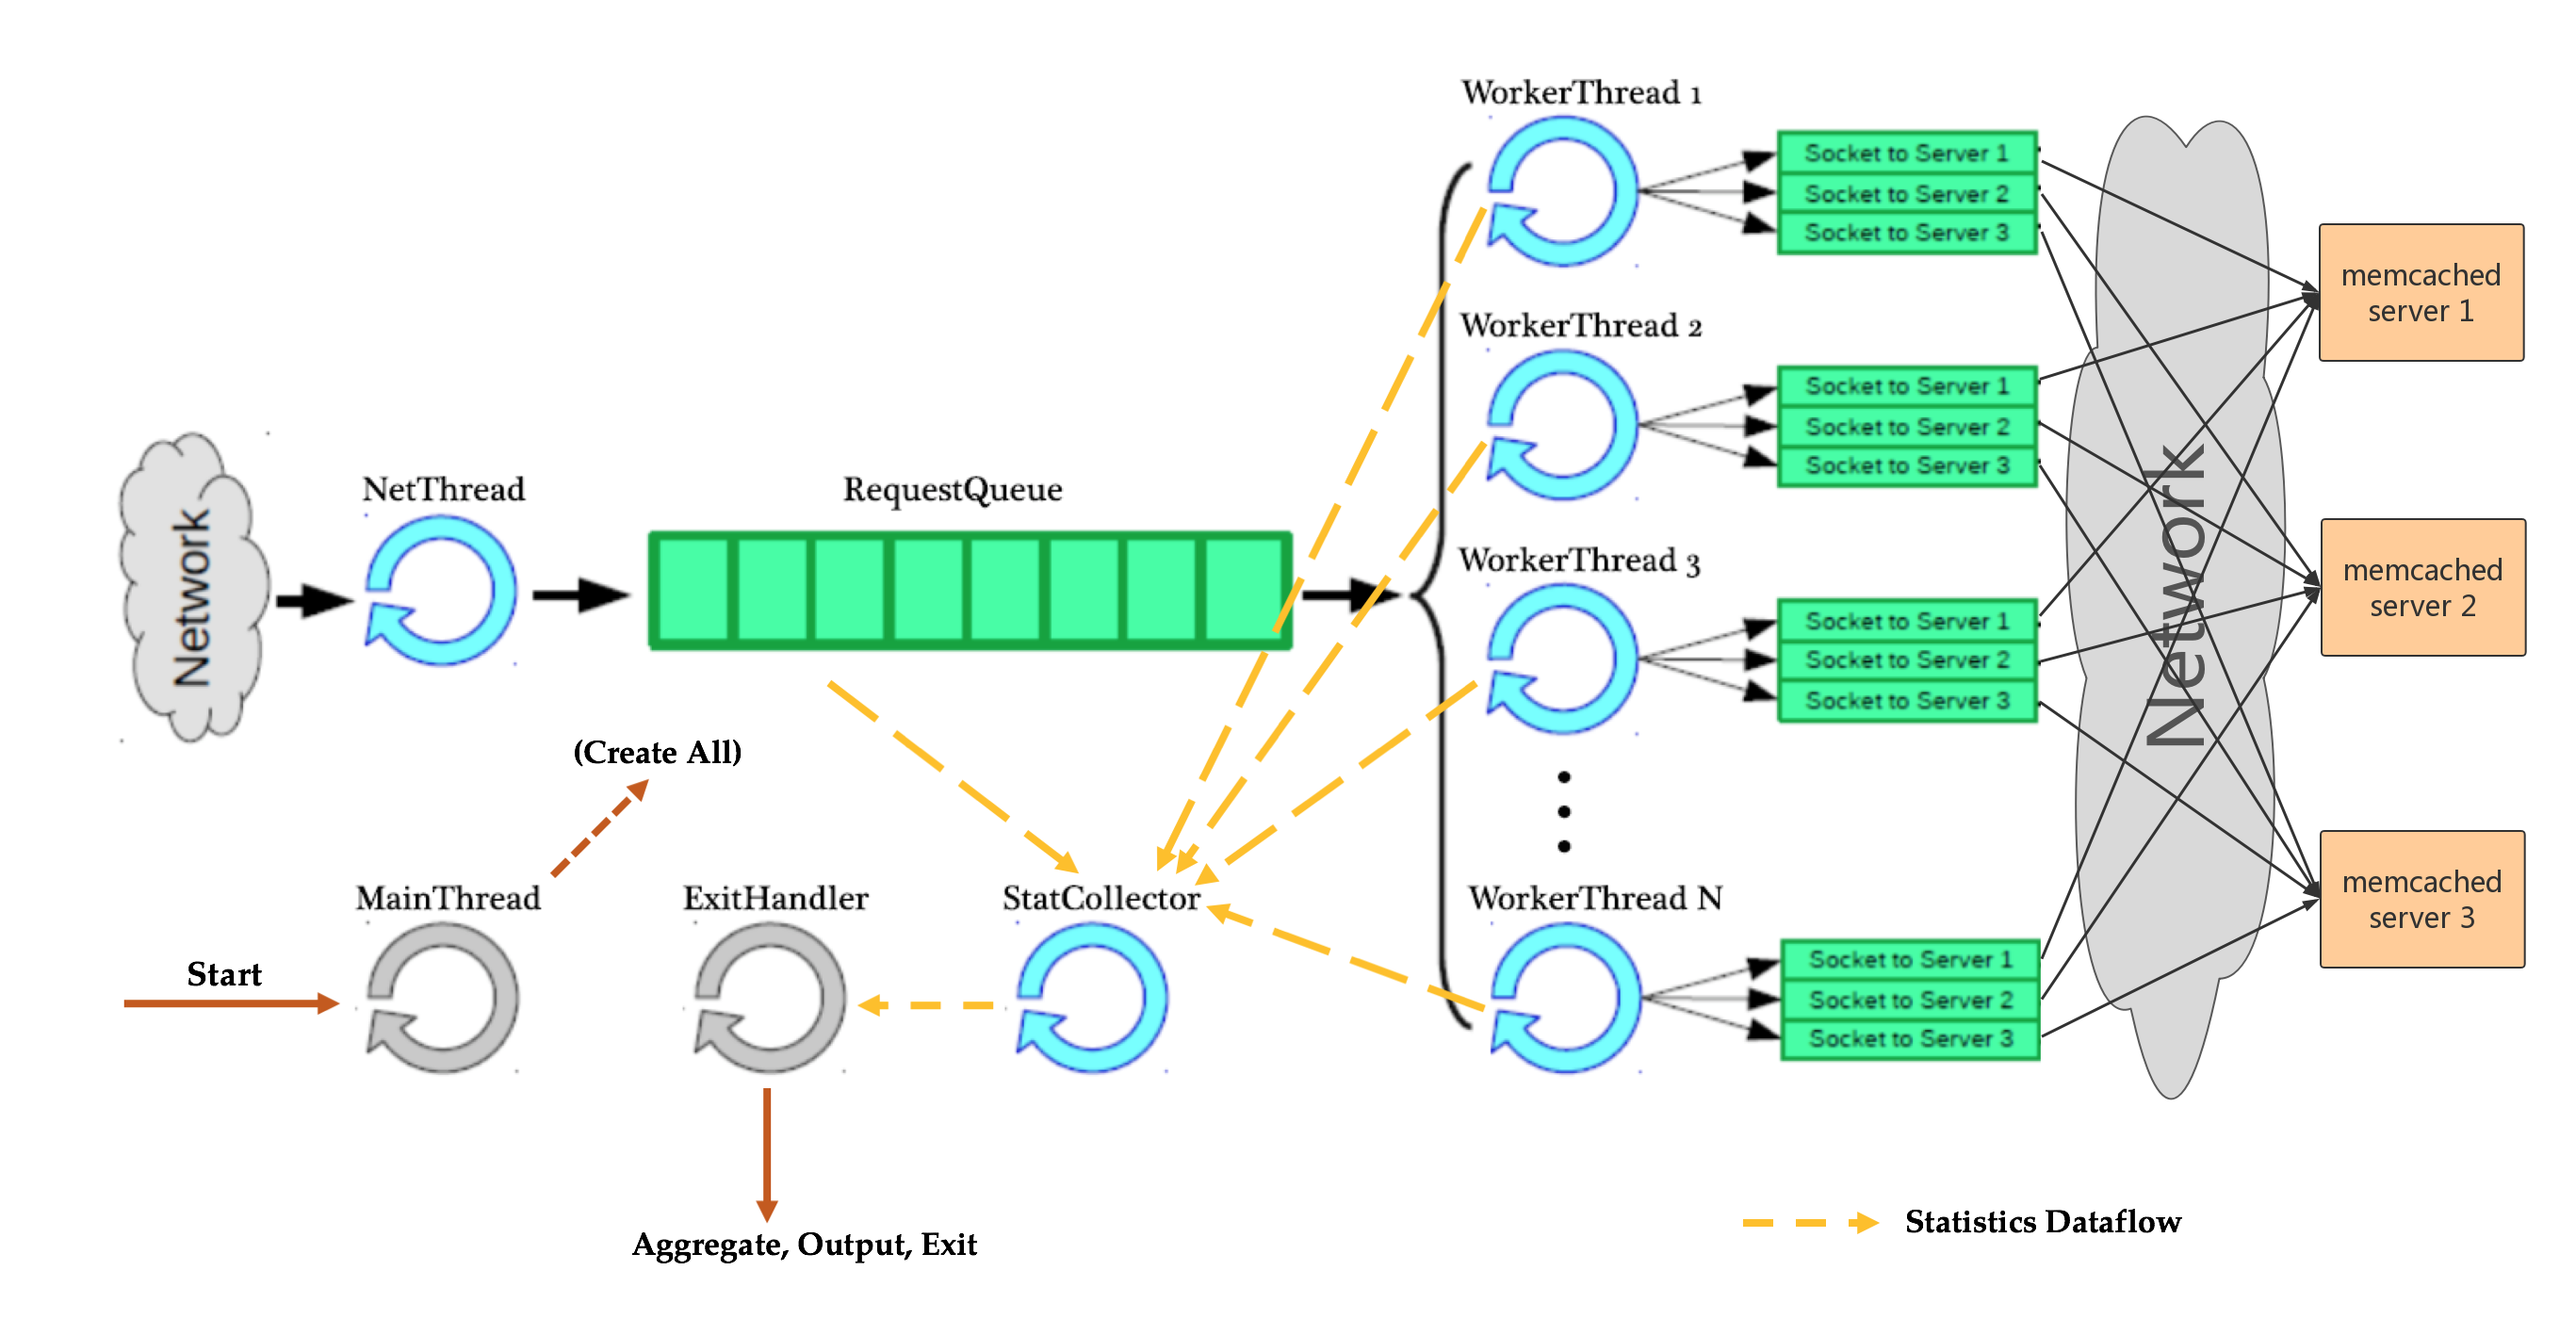
\includegraphics[width=1.0\textwidth]{img/1_System_Architecture.png}
\caption{\label{fig:architecture}Multi-threaded Middleware Architecture}
\end{figure}

\subsubsection{Java Classes Functionality and Implementation} \label{java_class_diagram}

The middleware is implemented in a number of classes, which can be classified into three categories and explained as below:

\noindent\textbf{\uppercase\expandafter{\romannumeral1}. Queueing and Networking}

\begin{enumerate}[noitemsep,topsep=0pt]
\item \texttt{MyMiddleware} - The main class of the middleware, where the \texttt{MainThread} starts. The main thread is the bootstrap thread on the middleware's startup, which dies dies after having done the following tasks in order:

\begin{enumerate}[noitemsep,topsep=0pt]
\item Parse the command line arguments to get the middleware's IP and port to listen on, the number of worker threads, the IP and ports of memcached servers, and whether to process multi-get requests in a sharded or non-sharded manner.
\item Create a request queue (a thread-safe blocking queue) to be shared among the network thread and all worker threads.
\item Create and start a number of \texttt{WorkerThread} threads, a \texttt{NetThread} thread, and a \texttt{StatCollector} thread, all of which sharing the same request queue created in the last step. The StatCollector thread is scheduled to collect the system's statistics data once a second.
\item Create an \texttt{ExitHandler} thread, and register it as a ShutdownHook of the JVM. That is, the ExitHandler will be and only be started when the virtual machine is going to shut down (for example, when the user sends a SIGINT signal by executing \texttt{kill -2 \$PID} to shut down the middleware).  
\end{enumerate}

After the main thread dies, and before the exit handler is executed, the middleware always has a network thread and a fixed number of worker threads running, plus a statistics collector thread started once a second.

\item \texttt{RequestQueue} - A wrapper of \texttt{java.util.concurrent.LinkedBlockingQueue}. An object of \texttt{RequestQueue} is shared among all worker threads, the network thread and the statistics collector thread. This queue maintains a total number of arrived requests on every \texttt{enqueue()}, which helps to compute the arrival rate in the \texttt{StatCollector} thread. Every time the method \texttt{getArrivalRate(duration)} is called, it returns the arrival rate calculated from the increment of arrivals since the last calculation, divided by \texttt{duration} seconds, which is the time elapsed since the last call. The queue also marks the enqueue time and dequeue time for a \texttt{Request} when it is enqueued or dequeued.

\item \texttt{Request} - A class representing the requests from clients. It keeps the following information of a request:
\begin{itemize}
\item the request content as a \texttt{String},
\item the request type as an \texttt{enum RequestType}, 
\item the number of keys in the request (only applicable for \texttt{GET}s and \texttt{MULTI-GET}s), 
\item all tokens of the request content split by spaces (only applicable for \texttt{MULTI-GET}s),
\item the \texttt{SocketChannel} of the client from which this request is sent, which is simply a reference to the \texttt{SocketChannel} used in the network thread,
\item six timepoints in microseconds ($\mu s$): when this request has completely arrived (\texttt{timeArrived}), when it has been enqueued by the network thread (\texttt{timeEnqueued}), dequeued by a worker thread (\texttt{timeDequeued}), sent to all corresponding servers (\texttt{timeSentToServers}), when the worker thread has received response from all servers (\texttt{timeServersResponded}), and when the worker has sent a response to the client (\texttt{timeSentToClient}).
\end{itemize}

\item \texttt{NetThread} - The network thread (\texttt{NetThread}) is the thread that listens on a local port, accepts incoming client connections to this port, reads \textbf{and parses} requests from clients and put them into the request queue. As one request may be split into more than one network packets, the network thread only enqueues a request when all packets of this request have been received. In order to recognize a completion of a request, the network thread needs to do parsing after each reading. It also parses a request to get some statistical information necessary for measuring instruments. The detailed parsing procedures are described in \ref{message_parsing}.

The communication functionality is implemented using \texttt{java.nio}. A \texttt{ServerSocketChannel} is created to listen for incoming connections, and one \texttt{SocketChannel} is established for each client connection. To listen for messages on all of these connections in a single network thread, all channels are registered to a \texttt{Selector} to perform non-blocking IO, selecting for \texttt{Acceptable} \texttt{ServerSocketChannel} or \texttt{Readable} \texttt{SocketChannel}s. When registering to the selector, every \texttt{SocketChannel} to client is attached with a \texttt{ByteBuffer}, which will be reused every time there is some message to be read on this channel. This avoids the overhead of allocating and deallocating \texttt{ByteBuffer}s on every message.

When the \texttt{ServerSocketChannel} is acceptable, which means there is a new client trying to connect to the middleware, a new \texttt{SocketChannel} is created to the new client. When a \texttt{SocketChannel} is readable, which means the client has sent a new message, the current timestamp is marked and \texttt{handleRead()} is called to parse the message; if the message forms a complete request, a \texttt{Request} is created and enqueued into the request queue with the marked arrival time. The parsing procedure is described in detail in \ref{message_parsing}.
\end{enumerate}

\noindent\textbf{\uppercase\expandafter{\romannumeral2}. Request Processing}

\begin{enumerate}[noitemsep,topsep=0pt]
\item \texttt{WorkerThread} - The worker thread, which is responsible for establishing its own socket connections to the memcached servers on start up, and extracting and processing requests one by one from the request queue using its own \texttt{RequestProcessor} instance. After a worker thread has successfully taken a request, it will first look at the request's type. If it is a \texttt{SET} or a \texttt{GET}, the worker will forward the request to one or more servers, wait for response(s), and send a final response back to the client. Otherwise, the worker will log this event and go on taking a next request without responding the client on this request. A worker thread will only take a next request after it has finished processing the current request. The detailed request processing procedures are described in \ref{request_processing}. The thread can be \texttt{interrupted} (e.g. when the shutdown hook is triggered), in which case it will stop taking new requests and terminate.  

\item \texttt{RequestProcessor} - An abstract class providing abstract method definitions and partial implementations for the request processing in a worker thread. There are two classes extending this abstract class: \texttt{NonShardedRequestProcessor} and \texttt{ShardedRequestProcessor}, between which the only difference is how \texttt{MULTI-GET} requests are processed. The methods for processing \texttt{SET}s and single-key or non-sharded \texttt{GET}s are implemented in \texttt{RequestProcessor} itself. 

Depending on the \texttt{readSharded} argument specified at startup, each worker thread creates its own \texttt{RequestProcessor} instance. The request processor is in charge of sending requests to all servers or in a round-robin manner, possibly re-assembling the request first (for the case of sharded \texttt{MULTI-GET}), as well as receiving responses from servers and sending responses to clients. The Socket IO with servers are wrapped by \texttt{BufferedReader}s and \texttt{PrintWriter}s. Sending to clients is backed by a single \texttt{ByteBuffer}, which is reused every time the request processor executes a \texttt{sendToClient(client, msg)}. Section \ref{request_processing} elaborates on how each type of requests is processed.

\item \texttt{NonShardedRequestProcessor} - The request processor extending \texttt{RequestProcessor} which implements \texttt{MULTI-GET} processing in a non-sharded way, which means multi-key \texttt{GET}s are tackled in exactly the same way as single-key \texttt{GET}s.

\item \texttt{ShardedRequestProcessor} \label{ShardedRequestProcessor} - The request processor extending \texttt{RequestProcessor} which implements \texttt{MULTI-GET} processing in a sharded way, which means multi-key \texttt{GET}s are splitted and distributed among more than one memcached servers, and responses are merged again into one before being forwarded to the client.  As the number of keys in each shard can be different, it also tries to balance the number of keys distributed to every server, by maintaining a priority queue of servers based on current total load, polling from the queue to get the least-loaded server, and sending the largest shard first. An empirical proof of balance is presented in \ref{balance_proof}.
\end{enumerate}

\noindent\textbf{\uppercase\expandafter{\romannumeral3}. Measuring Instruments}

\begin{enumerate}[noitemsep,topsep=0pt]
\item \label{Statistics} \texttt{Statistics} - Realtime statistics data with regard to all requests completed by one worker thread. Every worker updates its own \texttt{Statistics} on completion of every request, including the number of \texttt{SET}s, \texttt{GET}s, \texttt{MULTI-GET}s, total number of keys and misses in \texttt{GET}s and \texttt{MULTI-GET}s, the sums of waiting time, service time, response time and internal processing time (which equals to $\texttt{response} - \texttt{service} - \texttt{waiting}$) for each type, and the response time histograms for each type. Besides, after a thread has dequeued a request from the request queue, it will call \texttt{markQueueLength(oldLength)} to add to an accumulator the product of the old queue length and the time elapsed since this worker's last dequeuing, from which the average queue length estimated on this worker is derived later according to the definition of average queue length. 

The statistics collector thread will read every worker thread's \texttt{Statistics} once a second by calling \texttt{getThreadLog(duration)}, which will return a \texttt{ThreadLog} object containing the increments of all the sums, average throughputs of all request types and average queue length in the period between this call and last call, assuming the interval is \texttt{duration} seconds.


\item \texttt{ThreadLog} - The class of objects returned by \texttt{Statistics.getThreadLog(duration)}. It contains the statistics data of a worker thread within a period, as described in section \ref{Statistics}.

\item \texttt{PeriodLog} - Created in the statistics collector thread to hold the \texttt{ThreadLog}s  of a one-second period from all worker threads, as well as the arrival rate of the period, which is measured in the \texttt{RequestQueue}. Includes a \texttt{getMergedLog()} method, which returns a merged \texttt{ThreadLog} aggregating all workers' \texttt{ThreadLog}s it is holding. This method is called in the exit handler, when it is dumping the final statistics.

\item \texttt{StatCollector} - The body of the statistics collector (\texttt{StatCollector}) thread, a helper thread scheduled in a fixed rate (one second) by \texttt{ScheduledExecutorService}. Every time it is run, a new \texttt{PeriodLog} instance marked by the current second is created, and all workers' \texttt{ThreadLog}s generated by \texttt{Statistics.getThreadLog(period)}, as well as the arrival rate measured on the request queue, are put into the \texttt{PeriodLog}. The statistics it gathered are kept in the main memory, not outputted to the standard output until the exit handler thread does so before termination.

\item \texttt{ExitHandler} - The shutdown hook thread, registered as the JVM's \texttt{ShutdownHook} at startup. It is only run when the middleware is exiting, either by a user-pressed CTRL+C or by a SIGINT signal received by the JVM. It first interrupts the network thread and all worker threads, wait for all of them to stop, and then shutdown the executor of statistics collector. Before exiting, it dumps to the standard output the following statistics:

\begin{enumerate}[noitemsep,topsep=0pt]
\item All workers' statistics gathered by the statistics collector thread every one second, with a merged total statistics of every second.
\item A total statistics within the middleware's whole execution phase, merged from the statistics of all seconds, including the total number, average response time, maximum throughputs, average sizes, hits, misses, and miss rates (if applicable) for each type of requests.
\item Three response time histograms, in 0.1 millisecond steps, for \texttt{SET}, \texttt{GET}, \texttt{MULTI-GET} respectively, which are merged from the histograms of all threads.
\item All errors and exceptions occurred during the middleware's execution time.
\end{enumerate}

\end{enumerate}

\subsubsection{Thread Pool}

The network thread and worker threads in the middleware are manually created and started in the main thread, \textbf{without} using Java built-in \texttt{ThreadPool} or \texttt{Executor}. In case of failure on any thread, the whole system simply shuts down and return a \texttt{-1}, instead of creating a new thread to replace the failed thread. This keeps the system simple without compromising the required functionality.

The statistics collector thread is scheduled with Java's \texttt{ScheduledExecutorService}, which makes it easier to do the statistics collecting at a fixed rate. As the statistics collecting operation is trivial and fast, and we are starting the operation at the beginning of every second, we can safely assume that the interval of collecting operations is exactly one second.

\subsubsection{Message Parsing} \label{message_parsing}

Message parsing happens at two places in the middleware. The first is when a message from client is received in the network thread, as we need to know if it is a complete request or not, we have to parse the message. Additional information that is useful later, e.g. number of keys, tokenised commands, are also parsed and stored here by the way. The second is by the request processors of worker threads when reading responses, because we want to know if the full response has been received, how many keys are missed, or if any error has occurred. 

According to the memcached protocol, a request contains either a command line followed by a data block (for storage commands), or a command line only (for all other commands). Both the command line and the data block are terminated by ``\textbackslash r\textbackslash n". Similar formats applies for responses: for \texttt{GET} responses, there are zero or more items and an ``END\textbackslash r\textbackslash n" in the end, where an item is a command line followed by a data block, both terminated by ``\textbackslash r\textbackslash n"; for \texttt{SET} responses, there are only four possibilities: ``STORED\textbackslash r\textbackslash n", ``NOT\_STORED\textbackslash r\textbackslash n", ``EXISTS\textbackslash r\textbackslash n", ``NOT\_FOUND\textbackslash r\textbackslash n". We do not care about the response formats for other types of requests, since we only relay \texttt{SET}s, \texttt{GET}s and \texttt{GETS}es to memcached servers.

Parsing a request message involves the following steps. The assumption is that one read can get partial, exactly one, or more than one requests (which will not actually happen from memtier clients). So, after the network thread reads the message into the \texttt{ByteBuffer} attached to the corresponding \texttt{SocketChannel}, it repeatedly checks if the buffer contains a complete request, convert that part into a string, and move the remaining bytes to the beginning of the buffer with \texttt{buffer.compact()}. On a next \texttt{read()}, the new message will be put in the same buffer after the existing bytes, and the whole buffer is checked again from its beginning for complete requests. After each read, we keep extracting requests from the buffer until it is empty or only contains a partial request. Then, the parsing on this buffer is stopped until a new \texttt{read} into this buffer is performed.

To check for a complete request, we decode the whole buffer into a \texttt{String}, and look for the first ``\textbackslash r\textbackslash n" in the string. If it is not found, which indicates a incomplete request, the parsing stops. Otherwise, the string is split into space-separated tokens, and we the first token indicates its type. If it is a storage command\footnote{Storage commands in memcached includes \texttt{set}, \texttt{add}, \texttt{replace}, \texttt{append} and \texttt{prepend}. Although we actaully only process \texttt{SET} commands, it is good to know the category in order to apply different parsing procedures.}, we then parse the fifth token as an integer, which indicates the size of the following data block, and we expect (size + 2) more bytes in the string (because of the terminating ``\textbackslash r\textbackslash n"). Otherwise, we do not expect more bytes, but we still check if the command is a \texttt{GET}, and, if it is, count the number of keys in it. Finally, we put the request into the request queue, along with its type, number of keys, \texttt{SocketChannel} to client, and, if it is a multi-key \texttt{GET}, the split tokens we have already got from parsing, so that we do not have to tokenize the request message again for sharding. 

\label{parsing_response} The parsing of server responses is similar, but it does not involve directly manipulating a buffer, because we use \texttt{java.io.BufferedReader.readLine()} to get a line string directly. Parsing \texttt{SET} responses is trivial, as we only need to read one line. For \texttt{GET} or muti-key \texttt{GET} responses, first we read one line to see if it is an ``END\textbackslash r\textbackslash n" (we call it an \texttt{end line}). If it is not, it must be the text line of an item. Then we tokenize the line and read the data block size from the fourth token, and call \texttt{BufferedReader.read()} for (size + 2) times to get the complete data block and terminating characters. This process is repeated until it has read an end line. For responses to multi-get shards, the only difference is that the end line is discarded. All shard responses are combined with a final end line appended. Note that the line returned by \texttt{BufferedReader.readLine()} does not include the carriage return and line feed characters in the end, so they are appended to the end manually.

The above parsing procedure is designed to be correct and robust, but not extremely efficient. It could cause performance bottlenecks, which we will discuss in later chapters.

\subsubsection{Request Processing} \label{request_processing}

In the middleware, every request is processed by exactly one worker thread, by calling the corresponding request processing method of the worker's \texttt{RequestProcessor}. When \texttt{readSharded} is \texttt{true}, every worker thread creates a \texttt{ShardedRequestProcessor} sharing the worker's \texttt{Statistics} and \texttt{Socket}s to servers. Otherwise, a \texttt{NonShardedRequestProcessor} is created in the same way. Both of the two classes extend the \texttt{RequestProcessor} class, which implements the processing of \texttt{SET}s and \texttt{GET}s. The only difference is the implementations of \texttt{processMultiGet} method. Thus, below we introduce request processing in four cases: \texttt{SET}s, single-key \texttt{GET}s, non-sharded multi-key \texttt{GET}s and sharded multi-key \texttt{GET}s.

For a \texttt{SET} request, the \texttt{processSet} method of the request processor is called after the request is dequeued and the attribute \texttt{timeDequeued} is set in the request. In \texttt{processSet}, the following steps are executed:

\begin{enumerate}[noitemsep,topsep=0pt]
\item The request is sent to all servers by calling \texttt{sendToServer(serverId, requestMessage)} in a \texttt{for} loop.
\item The attribute \texttt{timeSentToServers} is set in the request.
\item The responses of all servers are read one by one by calling \texttt{readers[serverId].readLine()} in a \texttt{for} loop, as a \texttt{SET} response always consists of only one line.
\item The attribute \texttt{timeServerResponded} is set in the request.
\item Every response is checked if its content is ``STORED", which means no error has occurred. If so, set the final response to reference the first response, otherwise, set it to reference the first non-STORED response.
\item A ``\textbackslash r\textbackslash n'' is appended to the final response.
\item The final response is sent to the client by calling \texttt{sendToClient(channel, response)}.
\item The attribute \texttt{timeSentToClient} is set in the request.
\end{enumerate}

For a single-key \texttt{GET} request or a non-sharded \texttt{MULTI-GET} request, the \texttt{processGet} method of the request processor or the \texttt{processMultiGet} method of \texttt{NonShardedRequestProcessor}, respectively, is called, after the request is dequeued and the attribute \texttt{timeDequeued} is set in the request. Both methods in turn calls the \texttt{processGetImpl} method, which executes the following steps:

\begin{enumerate}[noitemsep,topsep=0pt]
\item The server to send the request to is determined by calling \texttt{getAndIncrementNextServerIndex()}, which returns a next server index in a round-robin manner.
\item The request is sent to the determined server by calling \texttt{sendToServer(serverId, requestMessage)}.
\item The attribute \texttt{timeSentToServers} is set in the request.
\item The response of the server is read by calling \texttt{readGetResponse(serverId)}, which follows the parsing procedure as described in \ref{parsing_response}. The number of misses is also updated in this process.
\item The attribute \texttt{timeServersResponded} is set in the request.
\item The final response is sent to the client by calling \texttt{sendToClient(channel, response)}.
\item The attribute \texttt{timeSentToClient} is set in the request.
\end{enumerate}

After \texttt{processGetImpl} has returned, the number of missed keys is added to the worker's statistics.


For a sharded \texttt{MULTI-GET} request, the \texttt{processMultiGet} method of \texttt{ShardedRequestProcessor} is called, after the request is dequeued and the attribute \texttt{timeDequeued} is set in the request. The request is then processed in the following steps:

\begin{enumerate}[noitemsep,topsep=0pt]
\item The number and size of shards are determined from the number of keys and servers: $ \texttt{numShards} = \min{(\texttt{numServers}, \texttt{numKeys})} $, $ \texttt{shardSize} = \texttt{numKeys} / \texttt{numShards} $. 

If (\texttt{numKeys} \% \texttt{numShards}) $\neq$ 0,  the sizes of first (\texttt{numKeys} \% \texttt{numShards}) shards are added by one.

\item Each shard of request is assembled from tokens into a string, and sent to the lowest-loaded server polled from the priority queue as described in \ref{java_class_diagram}: \hyperref[ShardedRequestProcessor]{\texttt{ShardedRequestProcessor}}.
\item The attribute \texttt{timeSentToServers} is set in the request.
\item The response of each involved server is read and appended to a \texttt{StringBuilder} for the final response in the same order as in sending, by calling \texttt{readMultiGetResponse(serverId)}, which follows the parsing procedure as described in \ref{parsing_response}. The number of misses is also updated in this process.
\item The attribute \texttt{timeServersResponded} is set in the request.
\item The final response is sent to the client by calling \texttt{sendToClient(channel, response)}.
\item The attribute \texttt{timeSentToClient} is set in the request.
\end{enumerate}

\subsubsection{Proof of Balanced Load Distribution for GETs and multi-GETs} \label{balance_proof}


\begin{figure}[!ht]
\parbox{.5\linewidth}{
\centering
\captionsetup{justification=centering}
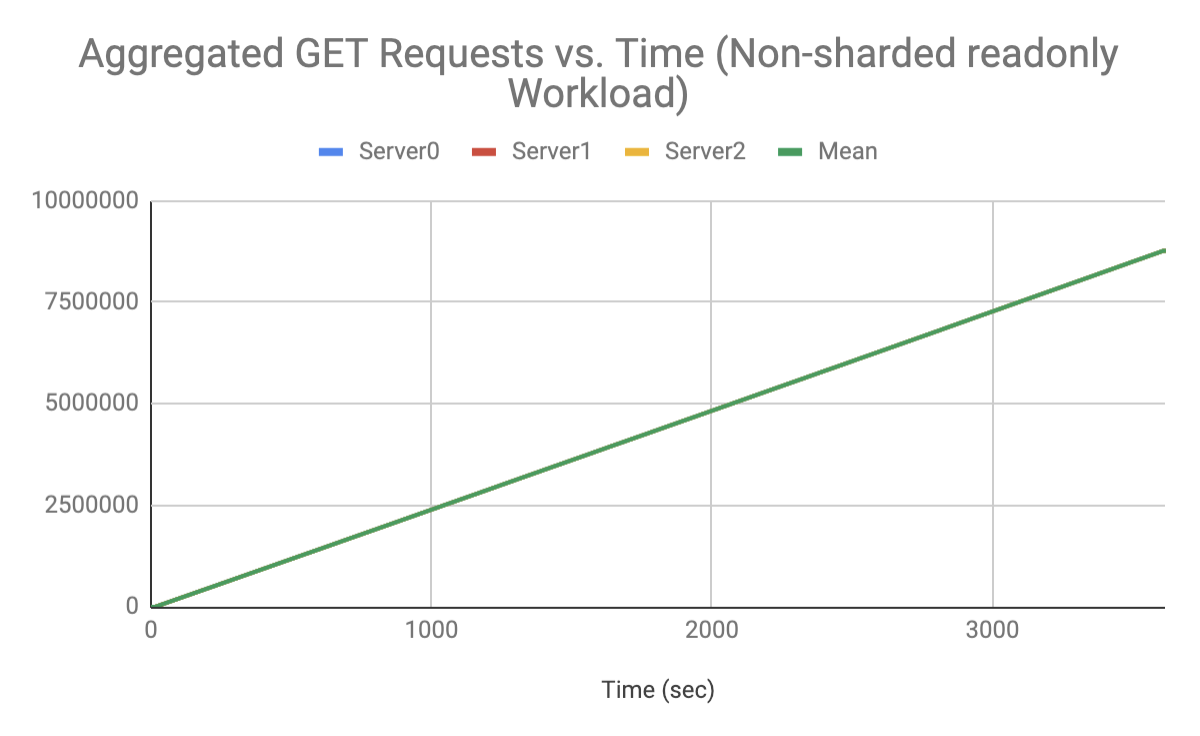
\includegraphics[width=0.5\textwidth]{img/1_get_aggregated.png}
\caption{\label{fig:load_distribution_get_aggregated}Load Distribution of GET \\(the lines are too close to be distinguished)}
}
\parbox{.5\linewidth}{
\centering
\captionsetup{justification=centering}
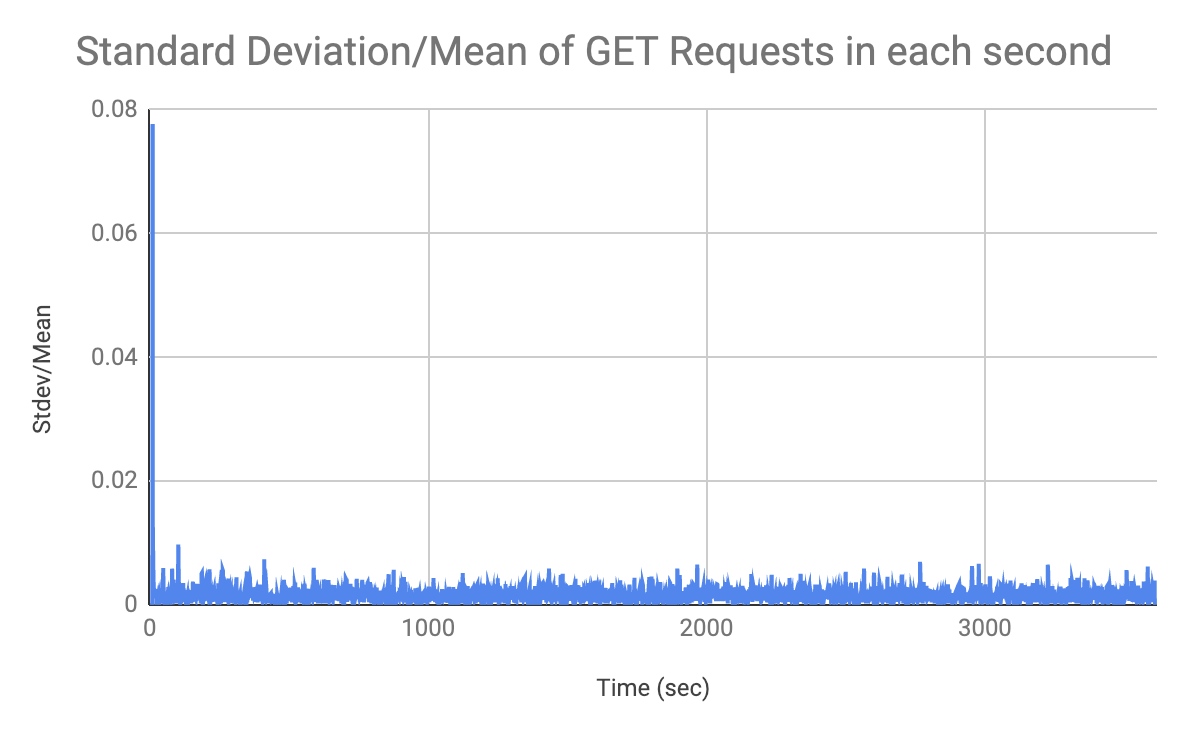
\includegraphics[width=0.5\textwidth]{img/1_get_stdev.png}
\caption{\label{fig:load_distribution_get_stdev}Standard Deviations of GET Load Distribution Per Second}
}
% \end{figure}

% \begin{figure}[!h]
\parbox{.5\linewidth}{
\centering
\captionsetup{justification=centering}
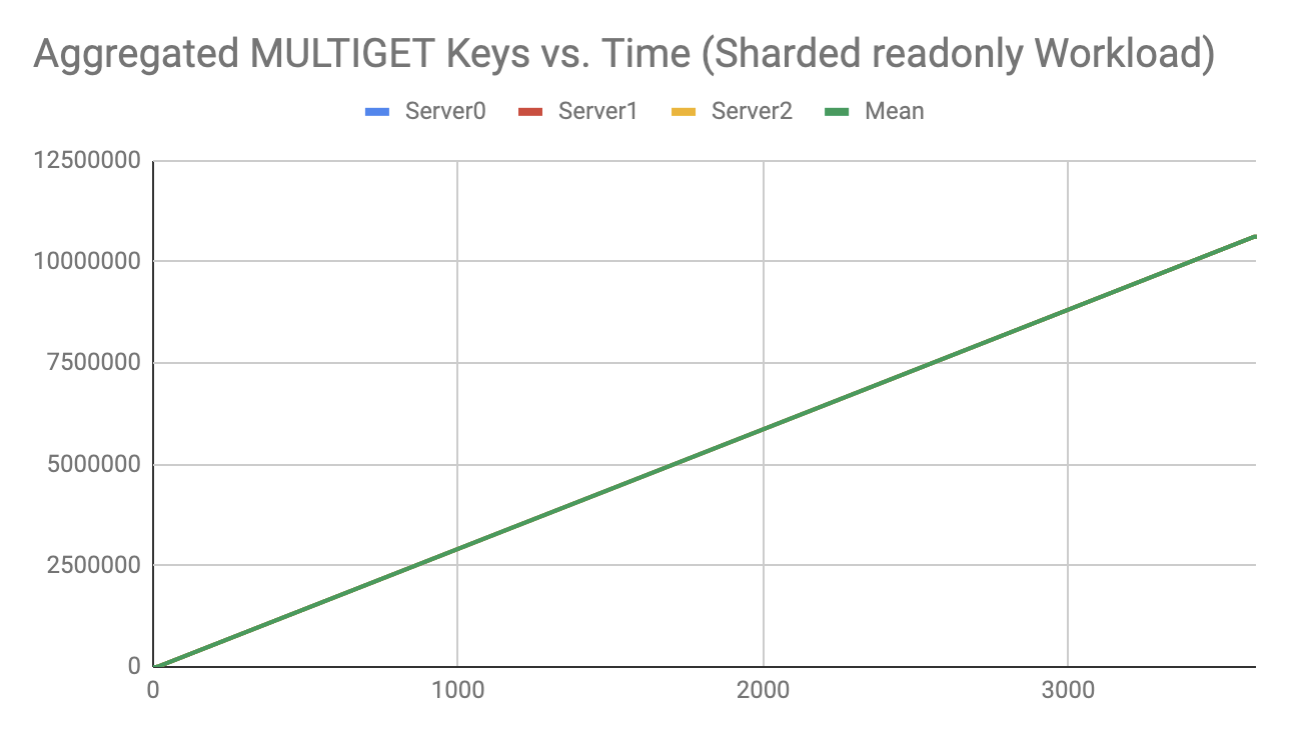
\includegraphics[width=0.5\textwidth]{img/1_multiget_aggregated.png}
\caption{\label{fig:load_distribution_multiget_aggregated}Load Distribution of MULTIGET \\(the lines are too close to be distinguished)}
}
\parbox{.5\linewidth}{
\centering
\captionsetup{justification=centering}
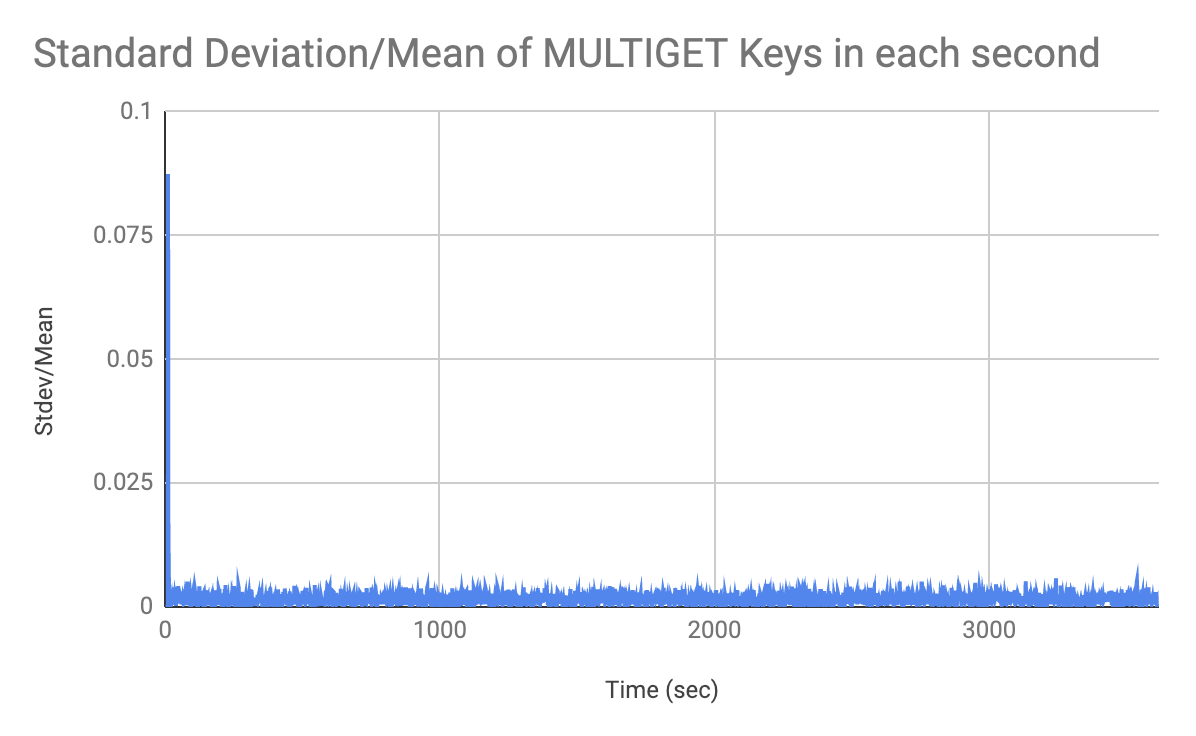
\includegraphics[width=0.5\textwidth]{img/1_multiget_stdev.png}
\caption{\label{fig:load_distribution_multiget_stdev}Standard Deviations of MULTIGET Load Distribution Per Second}
}
\end{figure}

The middleware tries to balance load among servers. This is trivial for \texttt{SET}s because they are naturally sent to all servers. For \texttt{GET}s, using a simple round-robin mechanism in each worker thread independently is sufficient, assuming that every worker has equal chance of dequeueing a request from the LinkedBlockingQueue. However, it is not easy to tell from the implementation of Java \texttt{LinkedBlockingQueue} whether it will release objects evenly among threads. Further, for \texttt{multi-GET}s, the shards may not be equal in size, and the request processor always generates larger shard first, therefore, simple round-robin can always distribute the largest shard to some server, resulting in an imbalance. Instead, a priority queue based on current number of keys of each server is used to get the lowest-loaded server every time when deciding each server to send.

To verify the balance distribution for \texttt{GET}s and \texttt{multi-GET}s, two one-hour readonly experiments was run with the following settings.

\begin{table}[ht]
\parbox{.5\linewidth}{
\centering
	\scriptsize{
		\begin{tabular}{|l|c|}
			\hline Number of servers                & 3                        \\ 
			\hline Number of client machines        & 1                        \\ 
			\hline Instances of memtier per machine & 1                        \\ 
			\hline Threads per memtier instance     & 2                        \\
			\hline Virtual clients per thread       & 32                  \\ 
			\hline Workload                         & Read-only \\
			\hline Multi-Get behavior               & N/A                      \\
			\hline Multi-Get size                   & N/A                      \\
			\hline Number of middlewares            & 1                     \\
			\hline Worker threads per middleware    & 64                      \\
			\hline Repetitions                      & 1                \\ 
            \hline Test time (seconds)              & 3600             \\
			\hline 
		\end{tabular}
	}
    \caption{Testing GET Distribution}
}
\parbox{.5\linewidth}{
\centering
	\scriptsize{
		\begin{tabular}{|l|c|}
			\hline Number of servers                & 3                        \\ 
			\hline Number of client machines        & 1                        \\ 
			\hline Instances of memtier per machine & 1                        \\ 
			\hline Threads per memtier instance     & 2                        \\
			\hline Virtual clients per thread       & 32                  \\ 
			\hline Workload                         & Read-only \\
			\hline Multi-Get behavior               & Sharded                  \\
			\hline Multi-Get size                   & 10                     \\
			\hline Number of middlewares            & 1                     \\
			\hline Worker threads per middleware    & 64                      \\
			\hline Repetitions                      & 1                \\ 
            \hline Test time (seconds)              & 3600             \\
			\hline 
		\end{tabular}
	} 
    \caption{Testing MULTIGET Distribution}
}
\end{table}



Figure~\ref{fig:load_distribution_get_aggregated} is the total number of \texttt{GET}s sent to each server as a function of total request numbers. The numbers at the end of the experiment are 8,768,473 for server 0, 8,768,443 for server 1, 8,768,424 for server 2, with a total of 45,812,372, an average of 8,768,446.667 and a standard deviation of 24.70. Figure~\ref{fig:load_distribution_get_stdev} is the standard deviations of the three servers' load divided by the mean load at each second. Since the standard deviation is no more than 0.1\% of the average, we can safely argue that the load for \texttt{GET}s is distributed evenly among servers. Similarly, Figures~\ref{fig:load_distribution_multiget_aggregated} and~\ref{fig:load_distribution_multiget_stdev} are for sharded \texttt{MULGIGET}s, with 10,620,038 keys for server 0, 10,620,013 for server 1, 10,619,995 for server 2, on average 10,620,015.33, and standard deviation 21.59, except that the units are keys instead of requests. 

Therefore, the \texttt{get} load is equally distributed among all servers, and the system is stable within a one-hour run.
